\chapter{Problem Analysis}
\label{cha:Problem Analysis}

\section{Lane Merging Problems}
\label{sec:Lane Merging Problems}
Vehicles may have to merge into another lane for a number of reasons. In this paper we focus on merges made at 'critical positions' such as junctions. This analysis could later be applied to merges made at non-critical points, though centralised approaches may struggle here.

\subsection{Single-to-Single Merge}
\label{subsec:Single-to-Single Merge}
A single-to-single merge (S2S merge) describes a situation where a vehicle moves from a single lane road into another single lane road, as seen in Figure \ref{fig:S2SMerge}. In this situation we label the lane that vehicles are moving from the 'current lane' (CL), and we label the lane that vehicles move to the 'target lane' (TL). We describe the vehicles that start on the CL as 'merging vehicles' (MV) and the vehicles that start on the TL as 'target vehicles' (TV). We have our critical position where the CL and TL connect.

\begin{figure}[htb]
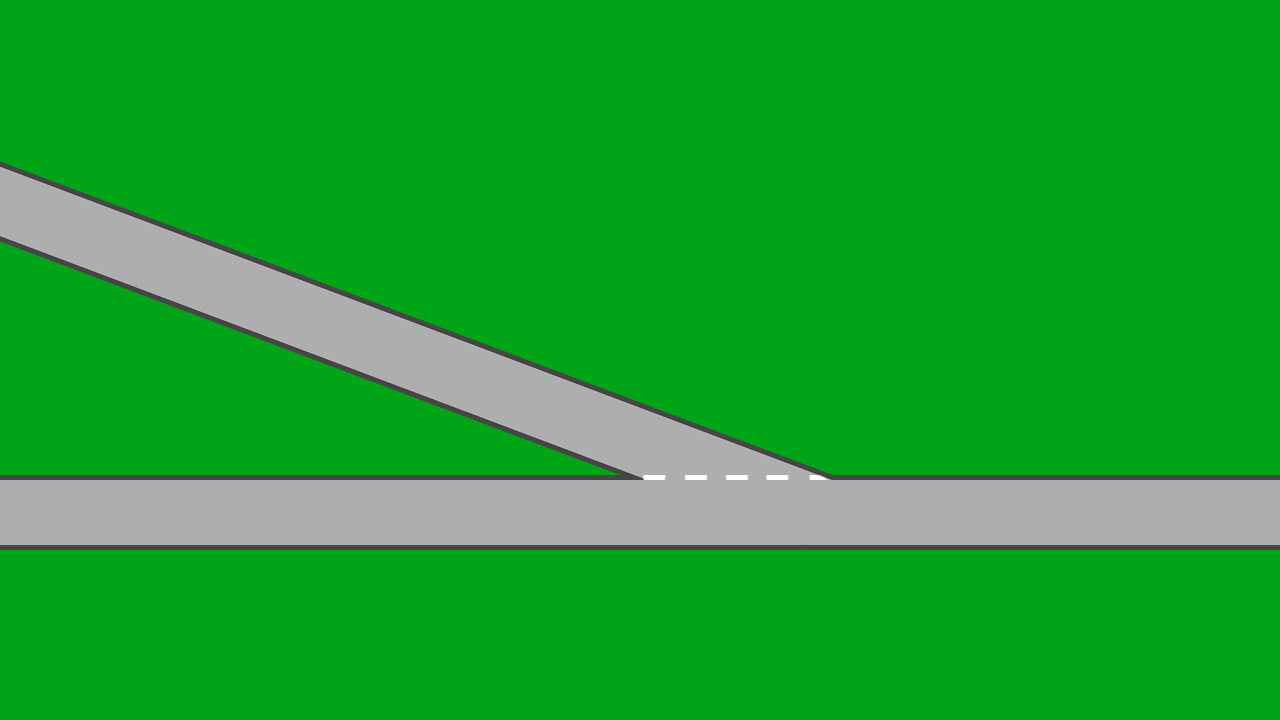
\includegraphics[width=\textwidth]{lane_diagrams/s2s.png}
\caption{A road with a single-to-single lane merge (S2S)}
\label{fig:S2SMerge}
\end{figure}

The main issue with an S2S merge stems from the limited options available to vehicles arriving at the critical position. Target vehicles do not have the opportunity to move laterally out of the way of merging vehicles, and vehicles on both lanes could struggle to reduce their velocity without affecting their successors.

\subsection{Single-to-Single Merge with slip-road}
\label{subsec:Single-to-Single Merge with slip-road}{}{}
\newtext{Many S2S merges are performed with an attached slip-road, as seen in Figure \ref{fig:S2SMergeExtended}.}

\begin{figure}[htb]{}
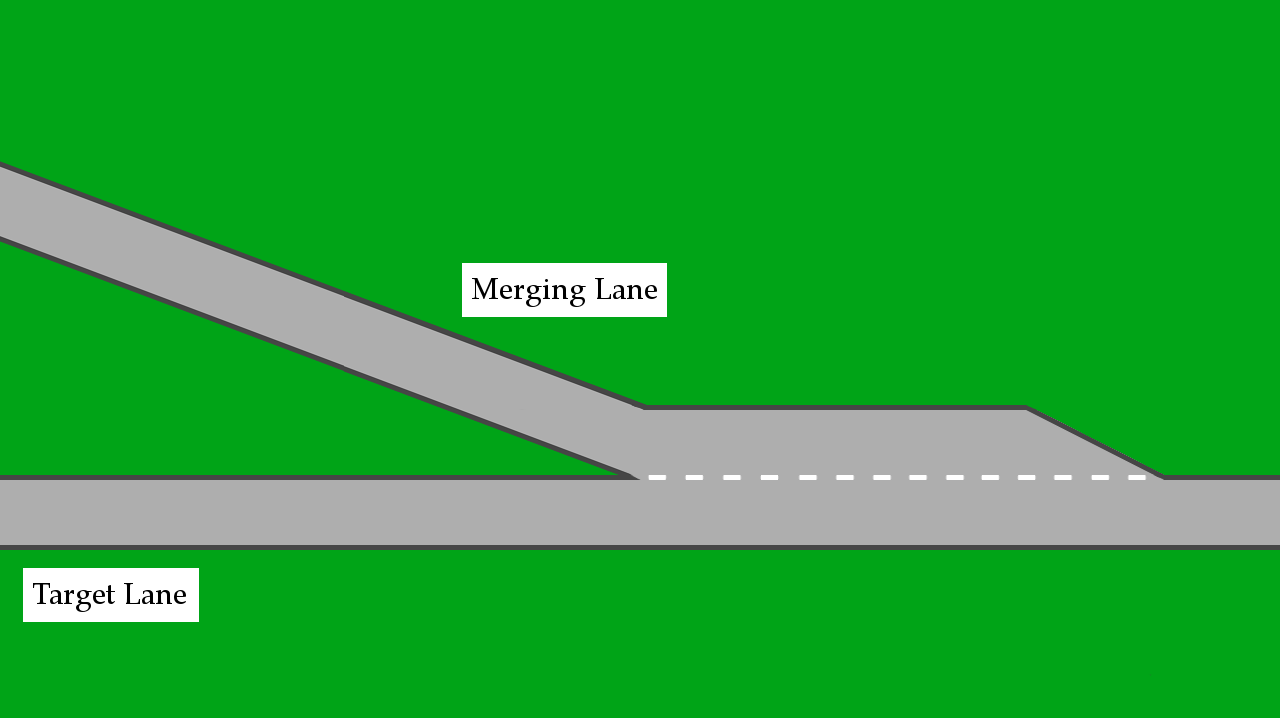
\includegraphics[width=\textwidth]{lane_diagrams/s2sExtended.png}
\caption{A road with a single-to-single lane merge and slip-lane (S2S)}
\label{fig:S2SMergeExtended}
\end{figure}

\newtext{The slip-road gives merging vehicles time to travel parallel to the target lane before merging. This makes the merge easier for both MVs and TVs as MVs don't slow down in front of TVs in order to make the turn into the TL. The effectiveness of slip-roads should change with length: the longer the slip-road, the more time MVs have to merge. This should improve the effectiveness of the merge position. We can vary the length of the slip-road to see how the performance of the merge changes.}

\subsection{Single-to-Double Merge}
\label{subsec:Single-to-Double Merge}
A single-to-double merge (S2D merge) describes a situation where a vehicle moves from a single lane road into a double lane road, as seen in Figure \ref{fig:S2DMerge}. In this situation we have two target lanes. The upper lane which directly links to the merging lane is called 'target lane 1' (TL1) and the lower lane is called 'target lane 2' (TL2). We still have only one critical position where the merging lane meets TL1.

\begin{figure}[htb]
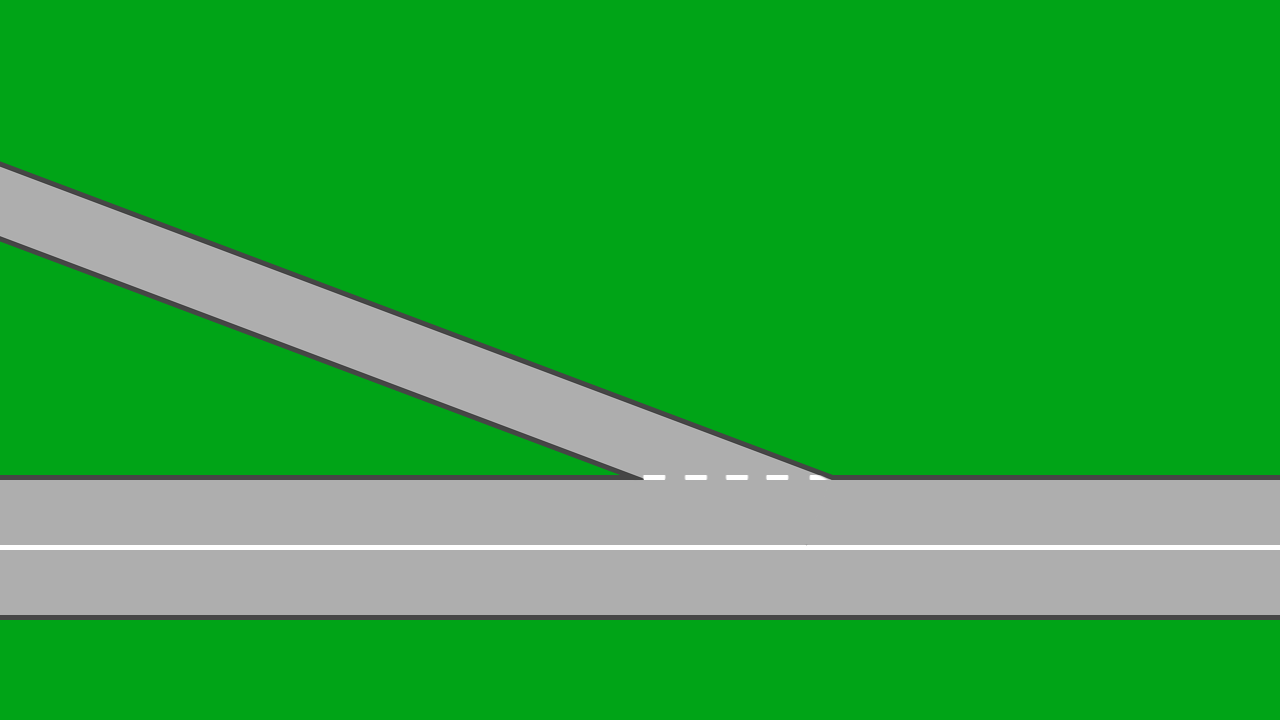
\includegraphics[width=\textwidth]{lane_diagrams/s2d.png}
\caption{A road with a single-to-double lane merge (S2D)}
\label{fig:S2DMerge}
\end{figure}

An S2D merge provides more options for vehicles on the targets lanes at the critical position. Target vehicles now have the opportunity to move laterally to avoid merging vehicles. Two lanes also allows for more vehicles on the target lane which should give vehicles greater freedom to adjust their velocity without affecting their successors.

\subsection{Single-to-Double Merge with slip-road}
\label{subsec:Single-to-Double Merge with slip-road}

\newtext{S2D merges can also take advantage of a slip-road, as seen in Figure \ref{fig:S2DMergeExtended}}

\begin{figure}[htb]
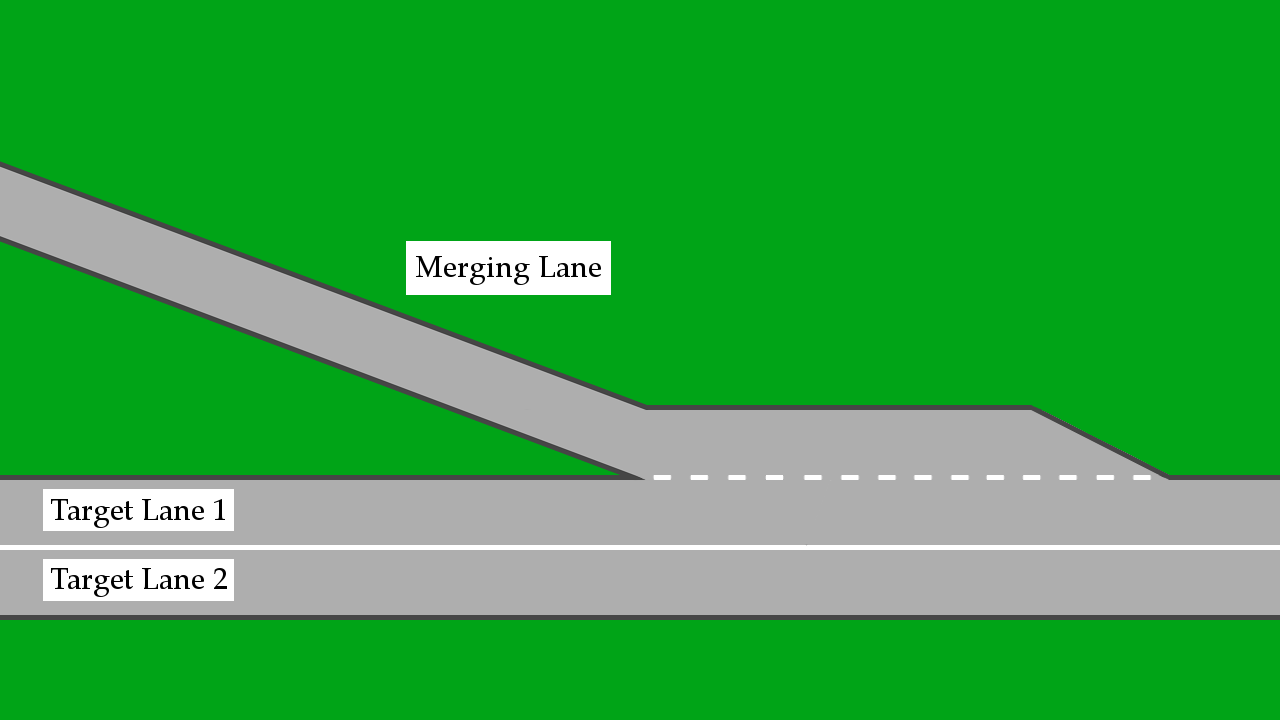
\includegraphics[width=\textwidth]{lane_diagrams/s2dExtended.png}
\caption{A road with a single-to-double lane merge and slip-lane (S2D)}
\label{fig:S2DMergeExtended}
\end{figure}

\subsection{Double-to-Double Merge}
\label{subsec:Double-to-Double Merge}
A double-to-double merge (D2D merge) describes a situation where a vehicle moves from a double lane road into another double lane road, as seen in Figure \ref{fig:D2DMerge}. We now have two merging lanes. The upper lane, 'merging lane 1' (ML1) merges into TL1 and the lower lane, 'merging lane 2' (ML2) merges into TL2.

\begin{figure}[htb]
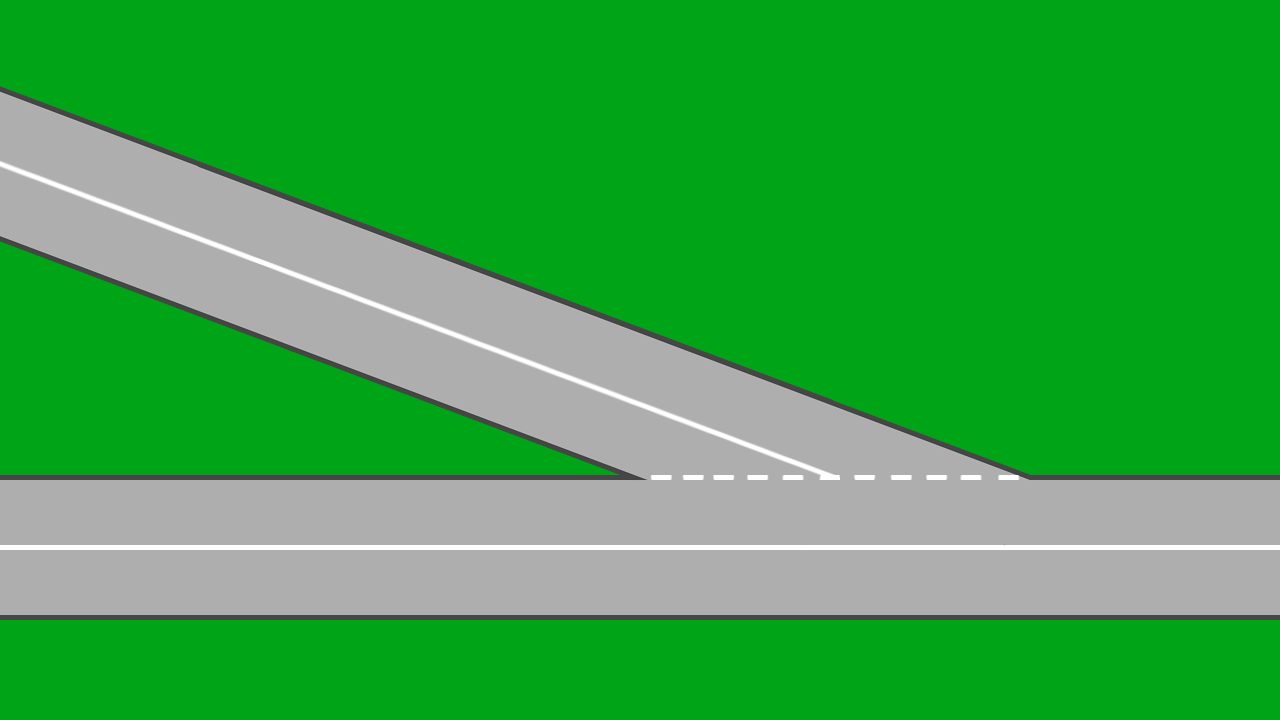
\includegraphics[width=\textwidth]{lane_diagrams/d2d.png}
\caption{A road with a double-to-double lane merge (D2D)}
\label{fig:D2DMerge}
\end{figure}

\newtext{With a D2D merge we now have to consider the effect of merging vehicles from ML2 driving across TL1. In addition, target vehicles can no longer laterally move out of the way of merging vehicles as they did before. Combining these factors with the wider range of options available to MVs, we can see that a D2D merge is far more complex than an S2D merge.}

\subsection{Double-to-Double Merge with slip-road}
\label{subsec:Double-to-Double Merge with slip-road}

\newtext{D2D merges can also take advantage of a slip-road, as seen in Figure \ref{fig:D2DMergeExtended}}

\begin{figure}[htb]
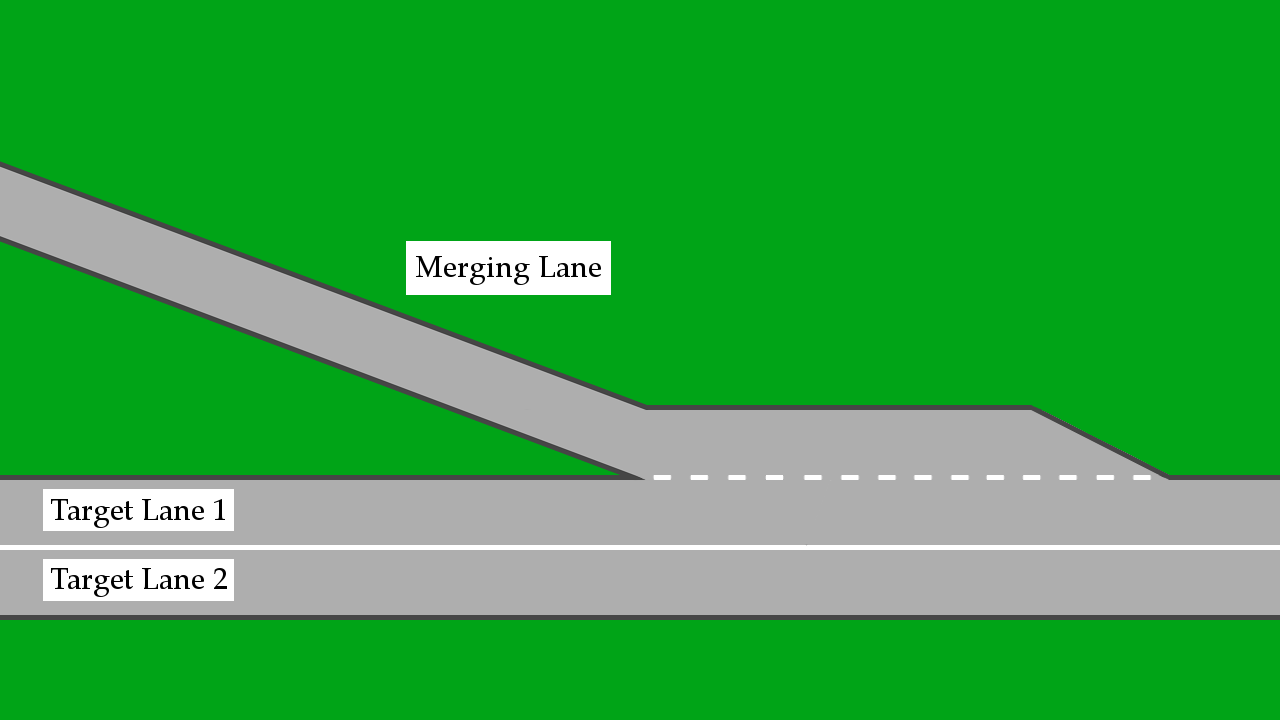
\includegraphics[width=\textwidth]{lane_diagrams/s2dExtended.png}
\caption{A road with a single-to-double lane merge and slip-lane (S2D)}
\label{fig:D2DMergeExtended}
\end{figure}

\newtext{D2D merges with a slip-road work differently to other slip-road schemes. In this instance vehicles on ML1 and ML2 will both merge into TL1. However, ML2 merges into TL1 as vehicles on an S2D merge would. ML1 vehicles merge into TL1 as vehicles on an S2D merge would when there is a slip-road in play.}

\subsection{Lane Obstruction Merge}
\label{subsec:Lane Obstruction Merge}
A lane obstruction merge is where a vehicle needs to change lanes to avoid an obstacle in their way, as seen in Figure \ref{fig:LaneObstruction}. It is essentially an S2S merge although the vehicle will tend to move laterally to avoid the obstacle. In this situation the critical position is the obstruction on the CL. 

\begin{figure}[htb]
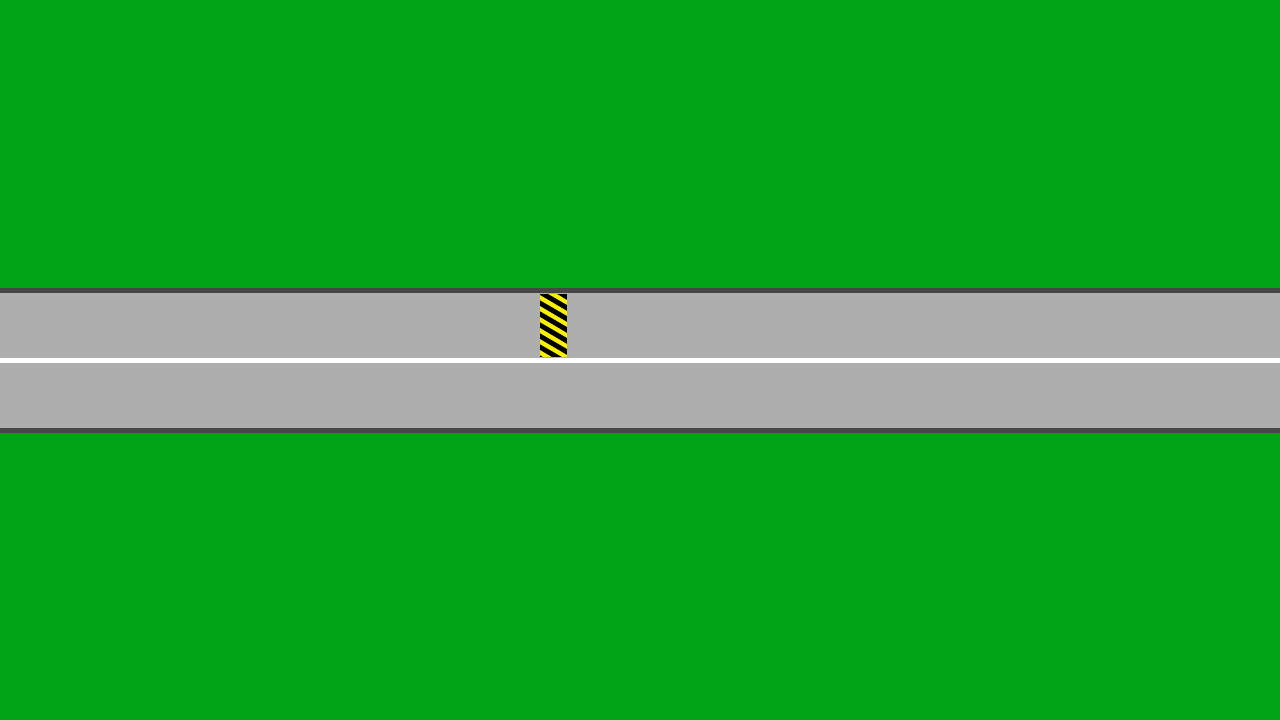
\includegraphics[width=\textwidth]{lane_diagrams/lane_blocker.png}
\caption{A road with a lane obstruction}
\label{fig:LaneObstruction}
\end{figure}

The obstacle could be a broken down vehicle or some debris on the road. Because of the unexpected nature of the obstacle it may sometimes be difficult to have a centralised approach to the problem. Although, if the obstacle was a broken down vehicle, the vehicle might be able to act as the centralised system managing approaching vehicles. 

\section{Measuring Success}
\label{sec:Measuring Success}
In order to evaluate the effectiveness of solutions to the problems we need to define measurements of success. 

Solutions to the merging problems above have to satisfy the following conditions:

\begin{enumerate}
\item \textit{No collisions}
This means avoiding collisions at the critical position between merging vehicles and target vehicles, as well as avoiding collisions between vehicles on the same lane.
\item \textit{Minimise delays to both lanes}
Vehicles should not suffer large delays to travel time due to the merge. \newtext{This means measuring both average delay and maximum delay. We do not want vehicles on one lane starving (not moving) for the benefit of vehicles on the other lane.}
\item \textit{Maximise throughput}
By minimising delays and velocity loss we aim to maximise the throughput of the critical position.
\item \textit{Minimise changes in velocity}
\newtext{Though not necessary, we should aim to minimises changes in vehicle velocity, for both passenger comfort and vehicle efficiency.}
\end{enumerate}

We need to measure how well solutions meet these conditions. 

\subsection{Collisions}
\label{subsec:Collisions}
Preventing collisions is a basic safety requirement for any autonomous vehicle system. We can measure this by comparing the positions of vehicles in the system, and ensuring that there is no overlap.

\newtext{We should also consider measuring near misses. We can define a minimum spacing between vehicles, perhaps equal to the minimum braking distance of the vehicle plus an additional comfort distance. This would mimic the IDM model \citep{Treiber2000}.}

Any collisions that do happen should be reported immediately. The system should automatically be considered a failure.

\subsection{Delay}
\label{subsec:Delay}
Delay measures the effect that the critical position had on the overall journey of the vehicle. It is the primary metric considered in Dresner et al.'s 2004 paper \citep{Dresner2004} on AIM. We will measure delay in a similar manner, calculating both average delay and maximum delay.

Dresner et al. provide the following equation for measuring average delay.

\begin{equation}
\frac{1}{|C|}\sum_{v_i\in{C}}\bigl(t(i) - t_0(i)\bigr)
\end{equation}

$C$ is the set of vehicles that pass through a critical position within a set time frame. Assuming no other vehicles on the road, a vehicle $v_i$ would complete it's trip in time $t_0(i)$, otherwise $v_i$ would complete it's trip in time $t(i)$. We can represent this trip for vehicles in the simulator as the time difference between the vehicle spawning in and the vehicle being removed from the simulator.

Dresner et al. also provide the following equation for measuring maximum worst case delay:

\begin{equation}
\max_{v_i\in{C}}\bigl({t(i)} - t_0(i)\bigr)
\end{equation}

\newtext{Measuring maximum delay (and minimising it) is important, as we do not want to have a solution where some vehicles have extremely large delay times and others have very low delay times. This should help avoid a 'starvation' situation where some vehicles never get to complete their trips.}

\subsection{Throughput}
\label{subsec:Throughput}
By minimising delay we should also maximise throughput; the two are closely related. However we should also collect direct metrics.

\begin{equation}
\text{Vehicle throughput} = \frac{|C|}{t}
\end{equation}

Here $t$ is the time it took for all of the vehicles in $C$ to pass through the critical position. If we want to measure the rate at which merging vehicles and target vehicles pass through the intersection separately we can change the definition of $C$ to reflect that.

\subsection{Velocity Changes}
\label{subsec:Velocity Changes}
\newtext{We want to reduce velocity changes as much as possible, aiming especially to eliminate rapid changes. Ideally autonomous vehicles should have very smooth acceleration and braking profiles. This both increases passenger comfort and improves fuel efficiency.}

\todo{Ask Lilian for ideas on best measurements.}

Current thoughts on measurement:

Maximum decleration: How to measure? Sample each second to see changes? More frequently than that? How large a sample is too big or too small?

Similar questions for maximum acceleration.

Should we also measure net velocity change over the whole critical position?